\begin{activite}[Proportionnalité ou pas ?]

\begin{center} 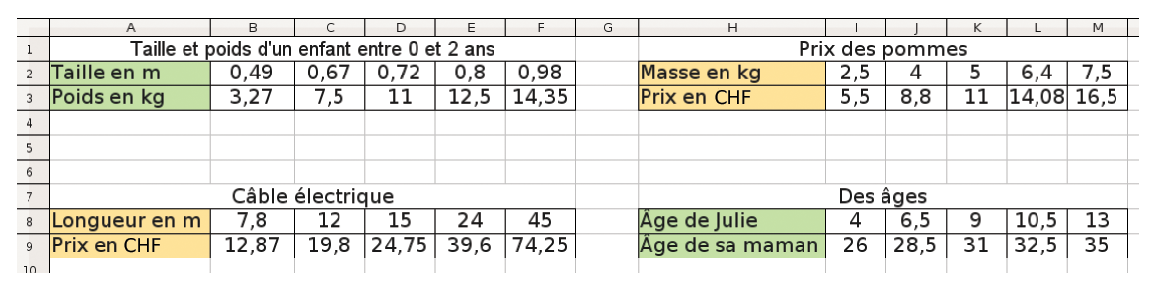
\includegraphics[width=15.8cm]{propor_pas} \end{center}

\begin{enumerate}
 \item Considère séparément chacun des tableaux. Les grandeurs comparées sont-elles \textbf{proportionnelles} ? \label{Propor_acti1}
 \item Note dans ton cahier le résultat de $B3 \div B2$ (tu peux utiliser ta calculatrice), puis le résultat de $C3 \div C2$, puis celui de $D3 \div D2$. Que peux-tu en conclure ?
 \item Fais les mêmes calculs pour les autres situations afin de vérifier tes réponses à la question \ref{Propor_acti1}.
 \item Réponds si possible aux questions suivantes.
 \begin{itemize}
  \item Quel sera le poids de l'enfant lorsqu'il mesurera 1 m ?
  \item Quel est le prix de 8 kg de pommes ?
  \item Quel est le prix de 35 m de câble électrique ?
  \item Quel sera l'âge de la maman lorsque Julie aura 17 ans ?
  \end{itemize}
 \end{enumerate}
 
\end{activite}

%%%%%%%%%%%%%%%%%%%%%%%%%%%%%%%%%%%%%%%%%%%%%%%%%%%%%%%%%%%%%%%%%%%%%%%%%

\begin{activite}[Et pour un ?]

Pour composer un lunch, un traiteur propose des toasts et du punch. Il prépare :
\begin{itemize}
 \item six toasts par personne ;
 \item des saladiers de punch de 5 l qui permettent de servir 40 verres chacun.
 \end{itemize}
 \begin{enumerate}
  \item Combien de toasts devra-t-il préparer pour une réception de 30 personnes ? De 45 personnes ? De 60 personnes ? De 75 personnes ?
  \item Un client lui dit : « 5 l pour 40 verres ? N'est-ce pas de trop petites rations ? » Comment faire pour le rassurer ?
  \item Chaque personne ne se servant qu’une fois, quelle quantité de punch le traiteur devra-t-il préparer pour une réception de 30 personnes ? De 45 personnes ? De 60 personnes ? De 75 personnes ?
  \item À la fin d’une réception, il reste 2 l de punch dans un saladier. Combien de verres le traiteur n’a-t-il pas servis ?
  \item Aide-le à réaliser un tableau avec lequel il pourra calculer le volume de punch à préparer pour un nombre de convives précis.
  \end{enumerate}

\end{activite}

%%%%%%%%%%%%%%%%%%%%%%%%%%%%%%%%%%%%%%%%%%%%%%%%%%%%%%%%%%%%%%%%%%%%%%%%%

\begin{activite}[Cœfficient de proportionnalité]

\begin{partie}[À la boulangerie]
\begin{minipage}[c]{0.68\linewidth}
La boulangère veut préparer une feuille de calcul pour lui permettre de déterminer plus rapidement le prix lors de la vente des croissants. \\[0.5em]
Fais un tableau contenant tous les prix de 2 à 10 croissants.
 \end{minipage} \hfill%
 \begin{minipage}[c]{0.28\linewidth}
  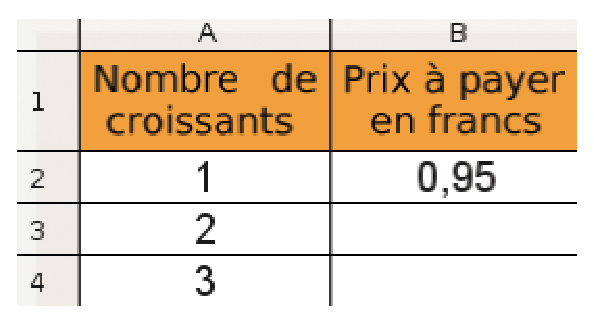
\includegraphics[width=4.2cm]{prix_croissant}
  \end{minipage} \\
\end{partie}

\begin{partie}[Comparaison de prix]
\begin{minipage}[c]{0.68\linewidth}
\begin{enumerate}
 \item À la station Seso, Rachid a acheté 43 l d'essence et a payé 41,71 CHF. Reproduis le tableau et détermine le prix que paiera Julia qui a mis 37 l d'essence dans son réservoir, sachant que le prix à payer est proportionnel au nombre de litres d'essence.
 \item Bruno, lui, a fait le plein de 48 l d'essence à la station Motal et a payé 44,64 CHF. À l'aide d'un tableau, réponds à la question suivante : Bruno aurait‑il dû aller à la même station que Rachid ?
 \end{enumerate}
 \end{minipage} \hfill%
 \begin{minipage}[c]{0.28\linewidth}
  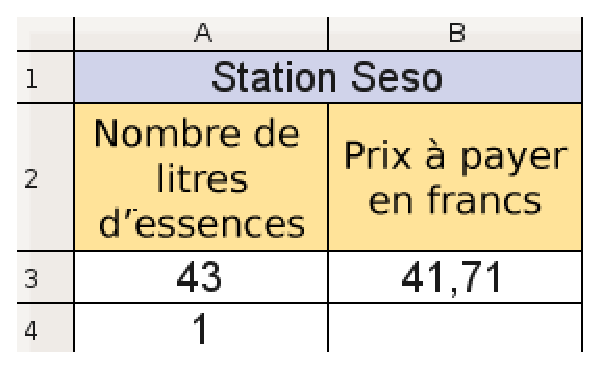
\includegraphics[width=4.2cm]{prix_essence}
  \end{minipage} \\
\end{partie}

\end{activite}

%%%%%%%%%%%%%%%%%%%%%%%%%%%%%%%%%%%%%%%%%%%%%%%%%%%%%%%%%%%%%%%%%%%%%%%%%

\begin{activite}[Premiers calculs]

Dans une jardinerie, la pancarte ci-dessous indique le nombre de sacs de graines à utiliser en fonction de la surface du terrain à ensemencer. \\[0.5em]

\begin{minipage}[c]{0.48\linewidth}
\begin{center} Terrain de 375 m\up{2} \end{center}
\vspace{0.3cm}
\begin{center} 
\includegraphics[width=2.2cm]{3sacs_gazon} \end{center}
 \end{minipage} \hfill%
 \begin{minipage}[c]{0.48\linewidth}
\begin{center} Terrain de 500 m\up{2} \end{center}
\vspace{0.3cm}
\begin{center} 
\includegraphics[width=2.2cm]{4sacs_gazon} \end{center}
  \end{minipage} \\

\begin{enumerate}  
 \item À l’aide de cette illustration, réponds aux questions suivantes :
 \begin{itemize}
  \item Quelle surface pourra ensemencer Jean-Paul avec 7 sacs ?
  \item Quelle surface pourra ensemencer Emmanuel avec 6 sacs ?
  \item De combien de sacs aura besoin Rachid pour réaliser une pelouse de 1\,500 m\up{2} ?
  \item Quelle surface pourra ensemencer Léonard avec 19 sacs ?
  \item Quelle surface pourra ensemencer Fatima avec 28 sacs ?
  \item De combien de sacs aura besoin Steeve pour réaliser une pelouse de 3\,875 m\up{2} ?
  \item Quelle surface pourra ensemencer Sonda avec 21 sacs ?
  \end{itemize}
 \item Trouve un moyen simple de présentation pour synthétiser ces questions et ces réponses.
 \item Propose plusieurs méthodes pour déterminer quelle surface de gazon on peut recouvrir avec un seul sac.
\end{enumerate}

\end{activite}

%%%%%%%%%%%%%%%%%%%%%%%%%%%%%%%%%%%%%%%%%%%%%%%%%%%%%%%%%%%%%%%%%%%%%%%%%

\begin{activite}[Recette de cuisine]

\begin{partie}
Pour faire un gâteau pour six personnes, il faut 150 g de sucre :
\begin{enumerate}
 \item Manon souhaite faire un gâteau deux fois moins gros. Quelle quantité de sucre doit‑elle utiliser ?
 \item Marine doit faire ce gâteau pour 9 personnes. Propose plusieurs façons de trouver la masse de sucre qu'elle doit utiliser.
 \item Sabrina dispose de 200 g de sucre. Détermine de plusieurs façons pour combien de personnes sera le gâteau.
 \end{enumerate}
\end{partie}

\begin{partie}
Les masses de farine et de sucre sont proportionnelles. Reproduis le tableau de proportionnalité et complète‑le le plus astucieusement possible : \\[0.5em]
\begin{center}
 \begin{tabularx}{0.7\linewidth}{|c|X|X|X|X|X|X|}
 \hline
\rowcolor{H3} Masse de sucre en g & 50 & 130 & 100 & 180 & 230 & 115 \\\hline
\rowcolor{F3} Masse de farine en g & 65 & 169 & & & & \\\hline
 \end{tabularx}
 \end{center}
\end{partie}

\end{activite}

%%%%%%%%%%%%%%%%%%%%%%%%%%%%%%%%%%%%%%%%%%%%%%%%%%%%%%%%%%%%%%%%%%%%%%%%%


